\documentclass[12pt, titlepage]{article}

\usepackage{booktabs}
\usepackage{tabularx}
\usepackage{hyperref}
\hypersetup{
    colorlinks,
    citecolor=blue,
    filecolor=black,
    linkcolor=red,
    urlcolor=blue
}
\usepackage[round]{natbib}
\usepackage{graphicx}
\usepackage{longtable}

%% Comments

\usepackage{color}

\newif\ifcomments\commentstrue %displays comments
%\newif\ifcomments\commentsfalse %so that comments do not display

\ifcomments
\newcommand{\authornote}[3]{\textcolor{#1}{[#3 ---#2]}}
\newcommand{\todo}[1]{\textcolor{red}{[TODO: #1]}}
\else
\newcommand{\authornote}[3]{}
\newcommand{\todo}[1]{}
\fi

\newcommand{\wss}[1]{\authornote{blue}{SS}{#1}} 
\newcommand{\plt}[1]{\authornote{magenta}{TPLT}{#1}} %For explanation of the template
\newcommand{\an}[1]{\authornote{cyan}{Author}{#1}}

%% Common Parts

\newcommand{\progname}{MTOBridge} % PUT YOUR PROGRAM NAME HERE
\newcommand{\authname}{Team 15, Alpha Software Solutions
\\ Badawy, Adham
\\ Yazdinia, Pedram
\\ Jandric, David
\\ Vakili, Farzad
\\ Vezina, Victor
\\ Chiu, Darren} % AUTHOR NAMES                  

\usepackage{hyperref}
    \hypersetup{colorlinks=true, linkcolor=blue, citecolor=blue, filecolor=blue,
                urlcolor=blue, unicode=false}
    \urlstyle{same}


\graphicspath{{images/}}

\begin{document}

\title{Project Title: System Verification and Validation Plan for \progname{}} 
\author{\authname}
\date{\today}
	
\maketitle

\pagenumbering{roman}

\section{Revision History}

\begin{tabularx}{\textwidth}{p{3cm}p{2cm}X}
\toprule {\bf Date} & {\bf Version} & {\bf Notes}\\
\midrule
October 30 & Darren & Non-Functional System Tests\\
November 1 & Pedram & Functional System Tests\\
November 1 & Victor & Unit Tests Intro\\
November 1 & Victor & Non-Functional System Tests\\
November 2 & Adham & Added Sections 3, 4.1, 4.2, 4.4, and 4.7\\
\bottomrule
\end{tabularx}

\newpage

\tableofcontents

\listoftables
\wss{Remove this section if it isn't needed}

\listoffigures
\wss{Remove this section if it isn't needed}

\newpage

\section{Symbols, Abbreviations and Acronyms}

\renewcommand{\arraystretch}{1.2}
\begin{tabular}{l l} 
  \toprule		
  \textbf{symbol} & \textbf{description}\\
  \midrule 
  T & Test\\
  \bottomrule
\end{tabular}\\

\wss{symbols, abbreviations or acronyms -- you can simply reference the SRS
  \citep{SRS} tables, if appropriate}

\newpage

\pagenumbering{arabic}

This document serves as a plan to verify and validate the design documents and outlines a series of system and unit tests for the functional and non functional requirements
of the program. It is intendd to be implemented as written, and for its results to be reported on in a future document.

\section{General Information}

\subsection{Summary}

The software whose Verification and Validation is planned for and referred to throughout this document is the User Interface component of MTO Bridge, 
a software developed in partnership with the Civil Engineering Department at McMaster university to assist MTO engineers in load rating bridges.
Its primary function is to present visually, in an intuitive and digestible way, the results of a simulation written by a Civil Engineering Professor and her lab 
in MATLAB of the forces imparted on a bridge by a platoon of trucks driving over it. There are two different solvers for two different results about the forces 
imparted on the bridge. The program will allow users to specify details of the bridge, the truck platoon driving over it, and which of the two results they are 
interested in knowing more about.\\ 

\subsection{Objectives}

There are two overarching objectives to any V\&V plan, ensuring we are actually building what we want to build correctly, or verification,
and ensuring that we think we want to build is what the client actually wants from us, or validation. Verification is where a lot of the domain specific definitions
of “correct” actually come in. As far as the verification plans for the design documents, the main goal is to build confidence that the design documents are complete,
verifiable, unambiguous, and generally of high quality. The design documents inform the implementation to a huge degree, so ensuring we are building on a solid foundation
is one of the main goals of this plan. As we are building a user interface, non functional qualities such as usability and performance/responsiveness are of 
utmost importance, and many of the tests outlined in this document will center around building confidence that our program has those qualities, or at least 
exposing if it doesn’t early on. As well, like any program, a number of our tests focus around ensuring that our program as written actually does what we think it does,
in a predictable way. Ensuring our program properly executes all the functions we laid out in the design documents, and nothing more or less.\\


\subsection{Relevant Documentation}

Essentially every design document written for this project will be relevant documentation here, a mostly exhaustive list of this would include:
\href{https://github.com/agentvv/MTOBridge/blob/main/docs/ProblemStatementAndGoals/ProblemStatement.pdf}{The Problem Statement}\\
\href{https://github.com/agentvv/MTOBridge/blob/main/docs/DevelopmentPlan/DevelopmentPlan.pdf}{The Development Plan}\\
\href{https://github.com/agentvv/MTOBridge/blob/main/docs/SRS/SRS.pdf}{The SRS}\\
\href{https://github.com/agentvv/MTOBridge/blob/main/docs/HazardAnalysis/HazardAnalysis.pdf}{The Hazard Analysis}\\
The Module Guide: This document is not yet written, but will be extremely relevant for this plan, particularly for unit testing\\
The Module Interface Spec: Same as the Module Guide.\\

\section{Plan}

The following section outlines a number of verification and validation plans for the design documents and the software. They are intended to act as a guide to be
carried out in order to verify the documents.
\\
\pagebreak
\subsection{Verification and Validation Team}

\begin{table}[hp]
  \caption{V\&V Team} \label{TblVnVTeam}
  \begin{tabularx}{\textwidth}{llX}
  \toprule
  \textbf{Name} & \textbf{Group} & \textbf{Role in V\&V}\\
  \midrule
  Adham Badawy& Dev Team & Developer, will conduct the bulk of the verification reviews and run System and Unit Tests\\
  David Jandric& Dev Team & Same as Adham Badawy\\
  Victor Vezina& Dev Team & Same as Adham Badawy\\
  Darren Chiu& Dev Team & Same as Adham Badawy\\
  Farzad Vakili& Dev Team & Same as Adham Badawy\\
  Pedram Yazdinia& Dev Team & Same as Adham Badawy\\
  Dr Yang Cancan& Client & Primary source for requirements elicitation and software validation inquiries\\
  Samuel Crawfod& Teaching Staff & Provides holistic verification reviews of design documents via a marking rubric\\
  
  \bottomrule
  \end{tabularx}
  \end{table}

\subsection{SRS Verification Plan}

For the SRS Verification, we will have a number of main goals, these are, in no particular order:
\begin{itemize}
\item Ensuring we have quality requirements
\item Ensuring our requirements are complete
\item Ensuring the document is free from grammar/spelling mistakes
\item Ensuring the document is legible/easy to understand
\end{itemize}
For ensuring the quality of the requirements, we will conduct a number of reviews with a number of different objectives. The primary reviews will be conducted by
the development team ourselves. And will be split into three separate reviews that will have the same methodology, but different goals. These will be as follows
\begin{itemize}
\item Checking requirements for an appropriate level of abstraction
\item Checking requirements for testability/verifiability 
\item Checking requirements ambiguity
\end{itemize} 

Two members of the team will be assigned to each of the three reviews, a compromise between giving each task more than 1 set of eyes and maintaining a feasible schedule
for the review. There are, after all, many other parts of this plan to be implemented.  As well, these same criteria go for both the functional and non-functional requirements,
and both will be reviewed in one pass. The subgroups will then discuss their findings at a meeting where any necessary changes to the SRS will be discussed. External, 
more holistic reviews of quality will also be conducted by 2 other teams enrolled in the course as well as the teaching staff, and this feedback will also be discussed 
amongst the group.\\\\ For requirements completeness, much of the same methodology of document readthroughs and reviews will occur, however the goal will be to identify any 
missing functionality through the review. The creation of other documents, such as the Hazard Analysis, is also done with ensuring SRS completeness in mind. The process of 
drafting these documents can illuminate new requirements previously unnoticed. This is also where the client, the Civil Eng. team we are working with, can come in handy.
Of course, we based our requirements entirely off of discussions with them, however it is often said that people can’t tell you exactly what they want, however if you show
them something specific, they can tell you whether or not they want that. It is not expected that the client will read the entire document, but we plan to prepare a quick 
summary of the requirements and present it to them and get their feedback on if anything strikes them as missing/incorrect. Naturally the client will also play a huge role
in Software validation, but this will be discussed in Section 4.7. A final note on completeness, it is impossible to prove that the SRS is truly, 100\% complete, but our team’s
mindset is that if we do our due diligence, we should get 99\% of the way there, and the difference should be negligible.\\\\
Once again, for grammar/spelling the same methodology applies, however this review process will be entirely internal. 1-2 group members will be assigned to 
check the document and ensure no errors of this nature exist. This step, while simple, is still important for the understandability and disambiguation of the document.\\\\
Finally, the last goal with regards to the SRS; legibility and ease of understanding, is a very subjective one. The main idea here is that the document should present 
its information in as easy to digest a way as possible. Is related information located near to each other? Is there proper traceability between all parts of the document? 
Is the document easy to navigate? These are the kinds of questions that 1 group member will be assigned to answer. Once again, they will report their findings and any 
recommendations to the group in the nearest meeting to their completion of the review chronologically.

\subsection{Design Verification Plan}

MTO bridge is bringing value mainly through creating an accessible user-friendly platform for bridge engineers. Therefore, the associated usability verification process should be more elaborate and done with greater insistence. The second most important design aspect is anticipation of change since our development effort is limited by the number of team members as well as the duration of this course. As a result, it’s important to verify our design output accommodates for potential future alterations. In our list of design metrics anticipation of change is divided into two design metrics flexibility and maintainability.\\\\
List of design metrics (in order of priority):
\begin{itemize}
\item \textbf{Usability}: How user friendly the system is. \\
The Heuristic Evaluation checklist below will be used by some of our and Dr.Yang’s team members ( a group of 3 to 5 people) on a prototype which closely resembles the final product. Evaluators scrutinize individual elements according to the heuristics. They also examine how these fit into the overall design, clearly recording all issues encountered. In a future session Evaluators can collate results for analysis and suggest fixes.
    \begin{itemize}
    \item \textbf{Keep users informed about its status} appropriately and promptly. 
    \item\textbf{Show information in ways users understand } from how the real world operates, and in the users’ language.
    \item\textbf{Offer users control} and let them undo errors easily.
    \item\textbf{Be consistent} so users aren’t confused over what different words, icons, etc. mean.
    \item\textbf{Prevent errors –} a system should either avoid conditions where errors arise or warn users before they take risky actions (e.g., “Are you sure you want to do this?” messages).
    \item\textbf{Have visible information, instructions, etc. to let users recognize options, actions, etc.} instead of forcing them to rely on memory.
    \item\textbf{Be flexible } so experienced users find faster ways to attain goals.
    \item\textbf{Have no clutter}, containing only relevant information for current tasks.
    \item\textbf{Provide plain-language help} regarding errors and solutions.\\
    \end{itemize}
\item\textbf{Flexibility:} The ease of expanding the product with new feature sets and capabilities.\\
We shall refer the module guide (MG) and determine based on the stretch goals section of the problem statement and goals document the feasibility of decomposition as well as design flexibility.
For example, one of our stretch goals was the ability to draw two dimensional models of bridges and have analysis performed based on the sketches. Graphical additions of this sort which might be common for our application would require a software design that decouples the “view” component as much as possible from other components. Our second stretch goal was having a customizable UI, consequently our sub-architecture for the "view" component should accommodate for a plug-and-play behaviour. A team members and volunteer class members from a different group will be divided into two groups and each group is responsible for verification of flexibility of one stretch goal. They can provide us with feedback in separate meetings, after they were given time to examine our Module Guide, on whether our modular structure and overall architecture can facilitate for this design metric.\\
\item\textbf{Maintainability:} The ease of coding bug repairs and adding minor features.\\
Maintainability is greatly dependent on principles such as information hiding, code reusability and single-responsibility. The MG will be examined to particularly check for proper decomposition of modules and the “secrets” they hide through their interface. Base classes and inheritance should be utilized in cases where a general module can be decomposed into smaller sub-classes. The MIS (Module Interface Specification) shall be analyzed to ensure that every function is only responsible for doing one thing and if its other functionalities can be separated using new methods. Code inspections will be performed to identify repetitive logic and separate them using a helper function or class. The code inspections, MG and MIS analysis are going to be conducted by all team members. MG and MIS analysis will commence as soon as they are completed and code inspections begin when the first prototype is created. Each team member is going to be responsible for a component and its code inspection (same for MG and MIS assessments).
\end{itemize}

\subsection{Verification and Validation Plan Verification Plan}
Similar to other sections, the V\&V verification plan involves a set of reviews conducted by our team and others. The goals for these reviews will be as follows:
\begin{itemize}
\item Ensure the plan is complete
\item	Ensure the plan is unambiguous
\item	Ensure the plan is feasible
\item	Ensure the plan actually accomplishes the objectives it says it does
\end{itemize} 
For all of these reviews there are three major divisions for the document. Verification/Validation Plans, System Tests, and Unit Tests. These divisions exist as the definition
of “complete, unambiguous, and feasible” is likely to be different, or at least they might be achieved differently for each of these sections, particularly between the plans
and the tests. For the most part, all of these reviews will be completed by assigning 2 members of the group to each of the three sections, having them conduct their analysis,
and reporting their findings and recommendations for changes to the group at the nearest available meeting. The only exception to this general rule is that a more holistic 
and comprehensive single review will be performed by the teaching staff for the capstone course, and some feedback from 1-2 other groups will be generated as well. 
Some more detailed notes on each of the goals follows below.\\\\ As far as completeness, the main aim here is to ensure that the plans and tests as written, if executed,
would genuinely function as a comprehensive verification and validation of the program. As well, this plan should be entirely followable by a third party with no information
provided besides this document and a primer on how to execute the code perhaps. Similarly to the SRS verification, 100\% completeness can never be guaranteed no matter how many
reviews we do, but an effort to strive towards that goes a long way.\\\\ For ambiguity, this connects to what was talked about at the end of the completeness section. 
This plan is worthless if we can’t actually follow it and draw conclusions from it, so it needs to be clear what is to be done, how it is to be done, and what we should expect
to get out of it. Making the plan unambiguous also helps this document to serve as a reliable test of the program. That is, if there’s only one way to interpret the plans, 
and the document is well thought out, the plan should return mostly the same results if given the same input program and documents, every time.\\\\
Feasibility is simple, but important. There is always more testing that can be done, more through reviews that can be conducted, infinitely recursing verification plans
and plans to verify the plans and plans to verify those plans, but at a certain point the buck must stop and considerations for the fact that this plan is written
with the intent to actually be carried out to the tee by a group of students with time constraints and other priorities must be made. A balance must be struck between
accomplishing the objectives set out in this document to the best of our abilities, and not overestimating what those abilities actually are.\\\\ The last goal is somewhat
related to all three of the previous ones. It basically functions as a final review of the document following the other three to double check the entire document more
holistically. If the document is complete, unambiguous, and feasible, this goal is likely already accomplished, but a holistic review will both not take too much time to
complete following the information gathered from the previous three and also serve as a nice wrap up for the verification.

\subsection{Implementation Verification Plan}
\begin{itemize}
  \item\textbf{Development tests:} Conducted with unit and integration level testing verifying the specified behavior of the sub-assemblies on the Module Interface Specification. Refer to sections 5 and 6 of this document for a detailed plan of system and unit tests.
  \item\textbf{Prototype testing:} Conducted with prototypes that closely resemble the final product. Each prototype created will immediately undergo exploratory testing where a potential user which in this case can be one of Dr.Yang’s civil engineering students is encouraged to try different sections of the applications and complete specific tasks while being monitored by the developers taking notes. Prototype testing can be conducted on an individual part or on the completed system under any conditions.
  \item\textbf{Analysis:} Since much of the effort is front-end related static analyzers might not be effective. Code inspection will be done by other team members when new implementation is getting merged to the sourcecode by a developer. We are going to put in place Github’s merge validation mechanism where a developer should do a pull request so that their code can be validated by other team members before the new additions are submitted.
  
\end{itemize}

\subsection{Automated Testing and Verification Tools}
\textbf{Linter}\\
The IDEs we are using (Visual Studio and Visual Studio Code) have their own code linters, which are enabled by default.
We may consider using clang-tidy for error checking, as well as looking questionable code constructs. We will only use it if the standard IDE linting it not sufficient. This tool is fairly standard, with integration in many IDEs. We can also have it look for code that is against certain coding standards, for example Google coding conventions. In order to maintain consistent code formatting, we will use clang-format for formatting. Using this linter, we can also easily select a coding standard to follow, which will come from a file in our repo. Many IDEs also support the use of clang-format.\\\\
\textbf{Unit Testing Framework}\\
We will be using a combination of two testing libraries to test our code. The first is Qt Test, a testing library made specifically for the Qt GUI framework we will be using. This testing library will be used to test the GUI elements of our project.
The second testing library we will be using is Google Test. This library will allow us to test the other parts of our code in great detail, and offers many advanced features that we can use during development (report generation, death tests, automatic test discovery, etc.).\\\\
\textbf{Code Coverage Measuring Tools}\\
Since we will using GCC for compilation, we will be using GCOV to test our code coverage. We will use it as
it comes standard with GCC, and will hook in directly with our compilation.




\subsection{Software Validation Plan}

There will be multiple steps to validating our software, however they will all have the same goal. Answering this question:  Are we building/did we build what our client wanted
us to build, or has there been some terrible misunderstanding? Well, if there’s always only one goal, then why are there multiple steps? We plan to have the validation
process be a continuous one throughout the development of the project. Sure, we could wait till the program was mostly done and then only check with them once we had 
something concrete to show, but that can lead to catastrophic refactoring if it turns out we weren’t on the right track.\\\\ We already have biweekly meetings
scheduled with the client for the lifespan of the project, every Friday at 10:00-11:00am. In the earlier stages of the project, these served as requirements elicitation
meetings and an opportunity to deepen our understanding of the problem. Now that the project is well underway, however, these same meetings will switch to a primarily software
validation role. As we make progress on the project, and lock in design decisions, we can run them by our primary stakeholder to ensure our vision remains aligned with theirs
and make any relevant tweaks as necessary along the way, rather than all at once near the end. This keeps us flexible and avoids any nightmare “back to the drawing board” 
scenarios.\\\\ It was mentioned in section 4.2 that we plan on creating a summary of the main parts of the SRS and presenting to our client for a document verification purpose,
but this exact methodology in a slightly more general sense would work perfectly for software verification as well. Distill what we are currently doing into a presentable
set of ideas and receive feedback from the client on how well this solves their problem and how it could be improved/what to avoid.\\\\ The implementation of this
section of the V\&V plan may sound a little vague in comparison to others, and that’s because it is. It’s difficult to predict exactly how client meetings may affect our
next steps or even refactor our requirements entirely, so the best way to track and report on the implementation of this section is likely in a set of meeting minutes
from each of the biweekly meetings and subsequent team follow up meetings, cut down to include only relevant V\&V information, and stuck into the V\&V report.

\section{System Test Description}
	
\subsection{Tests for Functional Requirements}

Below are system tests for the functional requirements in the SRS for MTOBridge.
Each functional requirement has at least one system test. The identifiers follow a pattern of
functional requirement number, system test number. For example, FR1.ST2 refers to the second
system test for functional requirement 1.

\subsubsection{MATLAB}

\paragraph{MATLAB Communication}

\begin{enumerate}

  \item{FR1.ST1\\}

  Control: Automatic

  Initial State: None

  Input: None

  Output: MATLAB engine started

  Test Case Derivation: The first step in the communication is to get the MATLAB engine
  to start.

  How test will be performed: The test will instantiate our MATLAB engine wrapper.

  \item{FR1.ST2\\}

  Control: Automatic

  Initial State: None

  Input: Truck, Bridge, and Analysis configurations

  Output: Any result from standard out or standard error

  Test Case Derivation: We just need to confirm that the engine is processing our
  input in some way, whether it gives an error or not.

  How test will be performed: Start the MATLAB engine through our wrapper, create
  some default truck, bridge, and analysis configurations, and try to run the analysis.

\end{enumerate}

\subsubsection{Truck Configuration}

\paragraph{Truck Configuration Input}

\begin{enumerate}

  \item{FR2.ST1\\}

  Control: Automatic

  Initial State: GUI exists

  Input: Axle load, axle spacing, number of trucks, headway

  Output: GUI fields are filled

  Test Case Derivation: If the data of the input fields can be entered, then the user
  should also be able to fill in the fields.

  How test will be performed: Input fields will filled, and checked if they have the
  correct value.

  \item{FR2.ST2\\}

  Control: Automatic

  Initial State: GUI exists

  Input: Invalid axle load, axle spacing, number of trucks, headway

  Output: GUI fields are filled, highlighted as incorrect

  Test Case Derivation: The user should be able to enter data, but be informed if the
  entered information is invalid.

  How test will be performed: Input fields will filled with incorrect information, 
  and the fields should be highlighted as incorrect.

\end{enumerate}

\paragraph{Truck Platoon Visualization}

\begin{enumerate}

  \item{FR3.ST1\\}

  Control: Automatic

  Initial State: GUI exists

  Input: Valid truck configuration

  Output: A valid visualization of the truck platoon shown

  Test Case Derivation: If a valid truck configuration is given, the user should be able to
  visualize the truck platoon.

  How test will be performed: Given a valid truck configuration, a visualization will be generated.
  The visualization will be saved as a picture and compared to the expected visualization.

  \item{FR3.ST2\\}

  Control: Automatic

  Initial State: GUI exists

  Input: Invalid truck configuration

  Output: A message informing the user of an incorrect truck configuration

  Test Case Derivation: If an invalid truck configuration is given, the user should be informed
  that the visualization cannot be created without a valid truck configuration.

  How test will be performed: Given an invalid configuration, the program will not show
  a visualization, but a message informing the user that a visualization cannot be created/shown
  until the configuration is valid.

\end{enumerate}

\paragraph{Save Truck Configuration}

\begin{enumerate}

  \item{FR4.ST1\\}

  Control: Automatic

  Initial State: GUI exists

  Input: A truck configuration

  Output: A file with the correctly saved configuration

  Test Case Derivation: The program should be able to take the existing truck configuration and
  save it so that it can be loaded or used later.

  How test will be performed: Given a truck configuration, a file will be created. Its contents
  will be compared with the expected contents.

\end{enumerate}

\paragraph{Load Truck Configuration}

\begin{enumerate}

  \item{FR5.ST1\\}

  Control: Automatic

  Initial State: GUI exists, a truck configuration file exists

  Input: Truck configuration file

  Output: Truck configuration input fields will be filled correctly

  Test Case Derivation: After loading a previously saved truck configuration file, the configuration
  should apply and fill the input fields for the truck configuration.

  How test will be performed: Given a truck configuration, a file will be created. Its contents
  will be compared with the expected contents.

\end{enumerate}

\subsubsection{Bridge Configuration}

\paragraph{Bridge Configuration Input}

\begin{enumerate}

  \item{FR6.ST1\\}

  Control: Automatic
  
  Initial State: GUI exists
  
  Input: Number of spans, bridge length
  
  Output: GUI fields are filled
  
  Test Case Derivation: If the data of the input fields can be entered, then the user
  should also be able to fill in the fields.
  
  How test will be performed: Input fields will filled, and checked if they have the
  correct value.
  
  \item{FR6.ST2\\}
  
  Control: Automatic
  
  Initial State: GUI exists
  
  Input: Invalid number of spans, bridge length
  
  Output: GUI fields are filled, highlighted as incorrect
  
  Test Case Derivation: The user should be able to enter data, but be informed if the
  entered information is invalid.
  
  How test will be performed: Input fields will filled with incorrect information, 
  and the fields should be highlighted as incorrect.

\end{enumerate}

\paragraph{Bridge Visualization}

\begin{enumerate}
  
  \item{FR7.ST1\\}
  
  Control: Automatic
  
  Initial State: GUI exists
  
  Input: Valid bridge configuration
  
  Output: A valid visualization of the bridge shown
  
  Test Case Derivation: If a valid bridge configuration is given, the user should be able to
  visualize the bridge.
  
  How test will be performed: Given a valid bridge configuration, a visualization will be generated.
  The visualization will be saved as a picture and compared to the expected visualization.
  
  \item{FR7.ST2\\}
  
  Control: Automatic
  
  Initial State: GUI exists
  
  Input: Invalid bridge configuration
  
  Output: A message informing the user of an incorrect bridge configuration
  
  Test Case Derivation: If an invalid bridge configuration is given, the user should be informed
  that the visualization cannot be created without a valid bridge configuration.
  
  How test will be performed: Given an invalid configuration, the program will not show
  a visualization, but a message informing the user that a visualization cannot be created/shown
  until the configuration is valid.
  
\end{enumerate}

\paragraph{Save Bridge Configuration}

\begin{enumerate}

  \item{FR8.ST1\\}
  
  Control: Automatic
  
  Initial State: GUI exists
  
  Input: A bridge configuration
  
  Output: A file with the correctly saved configuration
  
  Test Case Derivation: The program should be able to take the existing bridge configuration and
  save it so that it can be loaded or used later.
  
  How test will be performed: Given a bridge configuration, a file will be created. Its contents
  will be compared with the expected contents.

\end{enumerate}

\paragraph{Load Bridge Configuration}

\begin{enumerate}
  
  \item{FR9.ST1\\}
  
  Control: Automatic
  
  Initial State: GUI exists, a bridge configuration file exists
  
  Input: Bridge configuration file
  
  Output: Bridge configuration input fields will be filled correctly
  
  Test Case Derivation: After loading a previously saved truck configuration file, the configuration
  should apply and fill the input fields for the truck configuration.
  
  How test will be performed: Given a bridge configuration, a file will be created. Its contents
  will be compared with the expected contents.

\end{enumerate}

\subsubsection{Solver Setup}

\paragraph{Solver Selection}

\begin{enumerate}

  \item{FR10.ST1\\}

  Control: Automatic
            
  Initial State: None
            
  Input: text input to indicate the desired solver 
            
  Output: Calculation results based on the selected solver

  Test Case Derivation: The current logic allows for calculation of the demand at different areas called concerened sections. These can show the forces for both a single section as well as the entire bridge. 

  How test will be performed: The test involves running a series of pre-determined calculation using both solvers and then comparing with the auotmaic output selecting one solver at a time. 
					
\end{enumerate}

\paragraph{Section of Concern}

\begin{enumerate}

  \item{FR11.ST1\\}

  Control: Automatic
            
  Initial State: None
            
  Input: text input to indicate the desired section 
            
  Output: Calculation results based on the selected section

  Test Case Derivation: The current logic allows for calculation of the demand at different areas called concerened sections. These can show the forces for both a single section as well as the entire bridge. 

  How test will be performed: Once the section is selected, the test is performed by executing different types of platoon and bridge characteristic to derive actual results. These results are validated and compared to the exepected results calculated through the engine only. 
					
\end{enumerate}

\paragraph{Discretization Length}

\begin{enumerate}

  \item{FR12.ST1\\}

Control: Automatic
					
Initial State: None
					
Input: text input to indicate the discretization length 
					
Output: Calculation results based on the defined length

Test Case Derivation: In order to use the second solver, the system requires information on the number of equally spaced parts of the bridge. 

How test will be performed: Using an array of discretization lengths, we can take advantage of the engine's efficiency to calculate the maximum demand force in different context and compare with our own expected results. 

\end{enumerate}

\paragraph{Force Type}

\begin{enumerate}

\item{FR13.ST1\\}

Control: Automatic
					
Initial State: None
					
Input: text input to indicate the desired force type  
					
Output: Calculation results based on the selected parameters 

Test Case Derivation: The current implmentation of the engine allows for calculation across shear, torsion and flexural resistance

How test will be performed: The test entails creating a series of bridge types with different truck platoons that can be tested for all force types such as shear, torsion and flexural. Each data test is manually fed into the engine to output an expected output. 
					
\item{FR13.ST2\\}

Control: Automatic
					
Initial State: None
					
Input: text input to indicate the desired moment  
					 
Output: Calculation results based on the selected parameters 

Test Case Derivation: The current implmentation of the engine allows for calculation using postivie and negative moment 

How test will be performed: The test will be performed by using our pool of pre-determined bridge and truck platoon configs to test for both positive and negative moment given a certain force type. 

\end{enumerate}

\subsubsection{Result Visualization}

\paragraph{Concerned Section Result Visualization}

\begin{enumerate}

\item{FR14.ST1\\}

Control: Automatic
				
Initial State: None
					
Input: calculations based on the concerened section 
					
Output: Animation and visualiation highlighting the resulting properties on the specified bridge and load 

Test Case Derivation: As one of the main purposes of the program, the visualization will be interactable to show various views

How test will be performed: Relying on the pre-determined and validated data, we will graph the visulizations of each through the system as well as manually through the data produced by the engine. We can then compare the the expected and actual result across all available views. 
			
\end{enumerate}

\paragraph{Critical Section Result Visualization}

\begin{enumerate}

\item{FR15.ST1\\}

Control: Automatic
					
Initial State: None
					
Input: calculations based on the discretization length 
					
Output:  Animation and visualiation highlighting the resulting properties on the specified bridge and load 

Test Case Derivation: As one of the main purposes of the program, the visualization will be interactable to show various views

How test will be performed: Relying on the pre-determined and validated data, we will graph the visulizations of each through the system as well as manually through the data produced by the engine. We can then compare the the expected and actual result across all available views. 

\end{enumerate}

\subsubsection{Exectution Flow Logging}

\paragraph{Report Generation}

\begin{enumerate}

\item{FR16.ST1\\}

Control: Automatic
					
Initial State: None
					
Input: text input to indicate logging flags 
					
Output: text output, "logs"

Test Case Derivation: With the engine built in another framework, its important to log every state change throughout the calculations as triggered by the system

How test will be performed: While running multiple calculations, the system is asked to comprehensively log the flow in the engine. The system will be interrupted at times to test the robustness as well. The resulting logs should be clearly highlighting the steps taken including any errors or warnings.
					
\end{enumerate}

\subsection{Tests for Nonfunctional Requirements}

\wss{The nonfunctional requirements for accuracy will likely just reference the
  appropriate functional tests from above.  The test cases should mention
  reporting the relative error for these tests.}

\wss{Tests related to usability could include conducting a usability test and
  survey.}

\subsubsection{Look and Feel Requirements}
		
\paragraph{Graphics Informative Value Test}

\begin{enumerate}

\item{NFR1.ST1\\}

Initial State: Bridge UI mockups containing graphic elements will be prepared

Type: Manual, Static

How test will be performed: Civil engineers will be presented with mockups and expected to identify what the graphic elements represent with at least 90\% accuracy. Refer to Figure \ref{fig:ui-mockup} for example UI mockup.

\end{enumerate}

\subsubsection{Usability and Humanity Requirements}
		
\paragraph{Intuitiveness Test}

\begin{enumerate}

\item{NFR2.ST1\\}

Initial State: Application is opened with no past data

Type: Manual, Dynamic

Input/Condition: User inputs

Output/Results: Bridge analysis within 5 minutes of introduction

How test will be performed: Civil engineer will be asked to provide inputs

\end{enumerate}
		
\paragraph{Display Resolution Test}

\begin{enumerate}

\item{NFR3.ST1\\}

Initial State: Application is opened

Type: Manual, Dynamic

Input/Condition: Application is running on a computer with 1280x720 display

Output/Results: All buttons and animation window remain visible and accessible

\item{NFR3.ST2\\}

Repeat test NFR.ST3 for 1366x768 display

\item{NFR3.ST3\\}

Repeat test NFR.ST3 for 1920x1080 display

\item{NFR3.ST4\\}

Repeat test NFR.ST3 for 2560x1440 display

\item{NFR3.ST5\\}

Repeat test NFR.ST3 for 3840x2160 display

\end{enumerate}

\paragraph{Text Resizing Test}

\begin{enumerate}

\item{NFR4.ST1\\}

Initial State: Application is opened with no past data

Type: Manual, Dynamic

Input/Condition: Font size setting is changed to display as 8pt

Output/Results: All buttons and animation window remain visible and accessible

\item{NFR4.ST2\\}

Repeat test NFR.ST8 with font size 16pt

\item{NFR4.ST3\\}

Repeat test NFR.ST8 with font size 24pt

\item{NFR4.ST4\\}

Repeat test NFR.ST8 with font size 32pt

\end{enumerate}

\paragraph{Ease of Installation Test}

\begin{enumerate}

\item{NFR5.ST1\\}

Initial State: Application is not installed

Type: Manual

Input/Condition: Application is downloaded and installed

Output/Results: Application is ready to use within 30 minutes

How test will be performed: By civil engineer

\end{enumerate}

\paragraph{Consistent UI Test}

\begin{enumerate}

\item{NFR6.ST1\\}

Initial State: Visually similar UI elements are grouped into categories by developers

Type: Manual, Static

Input/Condition: Civil engineer asked to associate UI elements with their respective categories

Output/Results: Civil engineer sorts at least 90\% of UI elements into their predefined categories

\end{enumerate}

\subsubsection{Performance Requirements}

\paragraph{UI Speed Test}

\begin{enumerate}

\item{NFR10.ST1\\}

Initial State: Application is opened with no past data

Type: Manual, Dynamic

Input/Condition: Application used to generate a small bridge analysis whose total execution time is at most \textcolor{red}{X} seconds

Output/Results: Total execution time will not exceed underlying MATLAB script's execution time by 10\%

\item{NFR10.ST2\\}

Initial State: Application is opened with no past data

Type: Manual, Dynamic

Input/Condition: Application used to generate a large bridge analysis whose total execution time is at least \textcolor{red}{Y} seconds

Output/Results: Total execution time will not exceed underlying MATLAB script's execution time by 10\%

\end{enumerate}

\subsubsection{Operational and Environmental Requirements}
		
\paragraph{User Computer Test}

\begin{enumerate}

\item{NFR12.ST1\\}

Initial State: Application is opened on expected users' computer

Type: Manual, Dynamic

Input/Condition: Application used to generate a small bridge analysis

Output/Results: Time needed on user computer will not exceed time needed on developer computers by 10\%(?)

How test will be performed: The bridge analysis configuration will be one whose total execution time is at most \textcolor{red}{X} seconds on developer computers

\item{NFR12.ST2\\}

Initial State: Application is opened on expected users' computer

Type: Manual, Dynamic

Input/Condition: Application used to generate a large bridge analysis

Output/Results: Time needed on user computer will not exceed time needed on developer computers by 10\%(?)

How test will be performed: The bridge analysis configuration will be one whose total execution time is at least \textcolor{red}{Y} seconds on developer computers

\end{enumerate}

\subsubsection{Maintainability and Support Requirements}
		
\paragraph{Ease of Maintenance Test}

\begin{enumerate}

\item{NFR13.ST1\\}

Type: Automatic, Static

Input/Condition: Measure code file length in lines

Output/Results: At least 75\% of files will contain 750 lines of code or less

How test will be performed: Clang-tidy linter

\item{NFR13.ST2\\}

Type: Automatic, Static

Input/Condition: Measure method length in lines

Output/Results: At least 75\% of methods will contain 75 lines of code or less

How test will be performed: Clang-tidy linter

\item{NFR13.ST3\\}

Type: Automatic, Static

Input/Condition: Measure length of code lines

Output/Results: At least 75\% of lines will contain \textcolor{red}{\bf 120} characters or less

How test will be performed: Clang-tidy linter

\item{NFR13.ST4\\}

Type: Automatic, Static

Input/Condition: Measure nesting depth of methods

Output/Results: At least 75\% of methods will have a maximum nesting depth of 5 or less

How test will be performed: Clang-tidy linter

\end{enumerate}

\subsection{Traceability Between Test Cases and Requirements}

\begin{longtable}{|p{0.2\textwidth} | p{0.8\textwidth}|}
  \caption{System Test Traceability}
  \label{TblSTTraceability}\\
  \hline
  \textbf{Requirement} & \textbf{System Tests}\\
  \hline
  NFR1 & NFR1.ST1\\
  \hline
  NFR2 & NFR2.ST1\\
  \hline
  NFR3 & NFR3.ST1, NFR3.ST2, NFR3.ST3, NFR3.ST4, NFR3.ST5\\
  \hline
  NFR4 & NFR4.ST1, NFR4.ST2, NFR4.ST3, NFR4.ST4\\
  \hline
  NFR5 & NFR5.ST1\\
  \hline
  NFR6 & NFR6.ST1\\
  \hline
  NFR7 & \\
  \hline
  NFR8 & \\
  \hline
  NFR9 & \\
  \hline
  NFR10 & NFR10.ST1, NFR10.ST2\\
  \hline
  NFR11 & \\
  \hline
  NFR12 & NFR12.ST1, NFR12.ST2\\
  \hline
  NFR13 & NFR13.ST1, NFR13.ST2, NFR13.ST3, NFR13.ST4\\
  \hline
  NFR14 & \\
  \hline
  NFR15 & \\
  \hline
\end{longtable}


\section{Unit Test Description}

As outlined in our \href{https://github.com/agentvv/MTOBridge/blob/main/docs/DevelopmentPlan/DevelopmentPlan.pdf}{Development Plan}, we will be using Qt Test and Google Test to conduct our unit testing. These testing frameworks will allow us to create and run unit tests quickly and easily.

\subsection{Unit Testing Scope}

\wss{What modules are outside of the scope.  If there are modules that are
  developed by someone else, then you would say here if you aren't planning on
  verifying them.  There may also be modules that are part of your software, but
  have a lower priority for verification than others.  If this is the case,
  explain your rationale for the ranking of module importance.}

\subsection{Tests for Functional Requirements}

\wss{Most of the verification will be through automated unit testing.  If
  appropriate specific modules can be verified by a non-testing based
  technique.  That can also be documented in this section.}

\subsubsection{Module 1}

\wss{Include a blurb here to explain why the subsections below cover the module.
  References to the MIS would be good.  You will want tests from a black box
  perspective and from a white box perspective.  Explain to the reader how the
  tests were selected.}

\begin{enumerate}

\item{test-id1\\}

Type: \wss{Functional, Dynamic, Manual, Automatic, Static etc. Most will
  be automatic}
					
Initial State: 
					
Input: 
					
Output: \wss{The expected result for the given inputs}

Test Case Derivation: \wss{Justify the expected value given in the Output field}

How test will be performed: 
					
\item{test-id2\\}

Type: \wss{Functional, Dynamic, Manual, Automatic, Static etc. Most will
  be automatic}
					
Initial State: 
					
Input: 
					
Output: \wss{The expected result for the given inputs}

Test Case Derivation: \wss{Justify the expected value given in the Output field}

How test will be performed: 

\item{...\\}
    
\end{enumerate}

\subsubsection{Module 2}

...

\subsection{Tests for Nonfunctional Requirements}

\wss{If there is a module that needs to be independently assessed for
  performance, those test cases can go here.  In some projects, planning for
  nonfunctional tests of units will not be that relevant.}

\wss{These tests may involve collecting performance data from previously
  mentioned functional tests.}

\subsubsection{Module ?}
		
\begin{enumerate}

\item{test-id1\\}

Type: \wss{Functional, Dynamic, Manual, Automatic, Static etc. Most will
  be automatic}
					
Initial State: 
					
Input/Condition: 
					
Output/Result: 
					
How test will be performed: 
					
\item{test-id2\\}

Type: Functional, Dynamic, Manual, Static etc.
					
Initial State: 
					
Input: 
					
Output: 
					
How test will be performed: 

\end{enumerate}

\subsubsection{Module ?}

...

\subsection{Traceability Between Test Cases and Modules}

\wss{Provide evidence that all of the modules have been considered.}
				
\bibliographystyle{plainnat}

\bibliography{../../refs/References}

\newpage

\section{Appendix}

This is where you can place additional information.

\begin{figure}[h]
  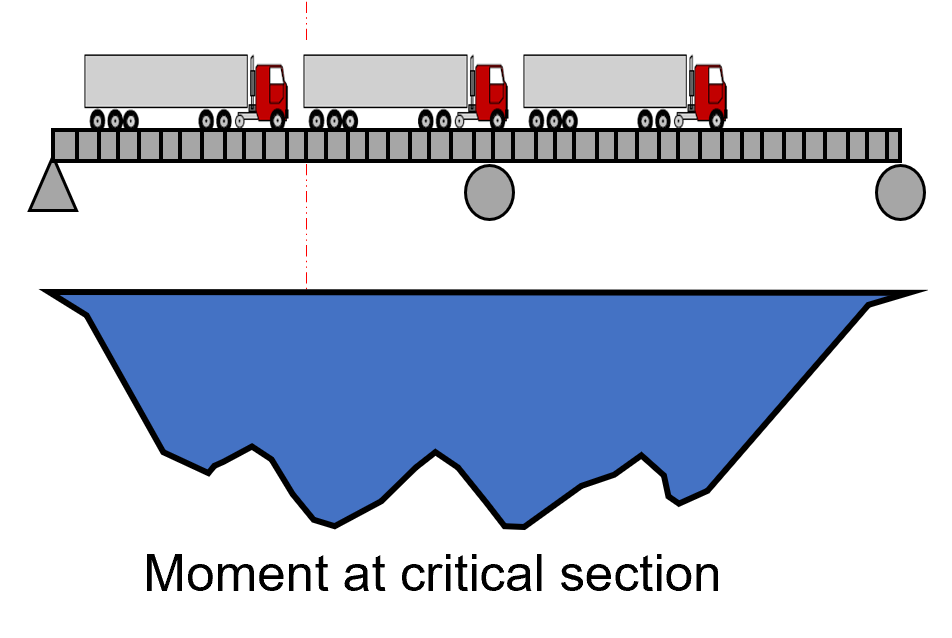
\includegraphics[width=\linewidth]{UI.png}
  \caption{UI mockup}
  \label {fig:ui-mockup}
\end{figure}

\subsection{Symbolic Parameters}

The definition of the test cases will call for SYMBOLIC\_CONSTANTS.
Their values are defined in this section for easy maintenance.

\subsection{Usability Survey Questions?}

\wss{This is a section that would be appropriate for some projects.}

\newpage{}
\section*{Appendix --- Reflection}

The information in this section will be used to evaluate the team members on the
graduate attribute of Lifelong Learning.  Please answer the following questions:

\begin{enumerate}
  \item What knowledge and skills will the team collectively need to acquire to
  successfully complete the verification and validation of your project?
  Examples of possible knowledge and skills include dynamic testing knowledge,
  static testing knowledge, specific tool usage etc.  You should look to
  identify at least one item for each team member.
  \item For each of the knowledge areas and skills identified in the previous
  question, what are at least two approaches to acquiring the knowledge or
  mastering the skill?  Of the identified approaches, which will each team
  member pursue, and why did they make this choice?
\end{enumerate}

\noindent\textbf{Darren}\\
\textbf{Most Important Learning(s):} We intend to use tools for validation including setting up CI/CD on the repo and clang-tidy for code analysis. Although I've used these or similar tools in the past, I haven't personally prepared them before.\\
\textbf{Plan to learn what is needed:} Some approaches for learning this is to research into the respective tools and reviewing past projects that used them, or to participate in their implementation and collaborate with team members on this. These aren't mutually exclusive, but I intend to mainly focus on learning through participating in the implementation and working with team members, since I feel that will be more effective in bringing results to the project.\\

\noindent\textbf{Adham}\\
\textbf{Most Important Learning(s):} My biggest blindspot with regards to the V\&V plan is the finer points of software testing, I think. While i am still relatively familiar
with concepts such as different types of testing, coverage metrics, and what have you, I'm definitely more than a little rusty.\\
\textbf{Plan to learn what is needed:} I still have access to my 3S03(software testing) slides, so I plan to use those to brush up on the concepts and techniques. As well,
there are a wealth of online videos and resources that I can use should i require more information than what was in my course. Primary source is definitely going to be the
slides, though. Probably slides-teammates-internet, in that order. \\

\noindent\textbf{David}\\
\textbf{Most Important Learning(s):} I think I need to learn a lot more about testing and test driven development.
Also I've never used a static analysis tool other than linters, so I need to learn what rules and static analysis
is necessary.
\textbf{Plan to learn what is needed:} To learn more about testing I'm going to look over some old course material,
and refer to online resources. I think I will also need to visit the documentation for Google Test because it's
a testing framework I've never used. To learn more about static analysis I think online resources will be the best
bet, and also visiting the documentation for clang-tidy will help with knowing the types of static analysis that
are available to us.\\

\end{document}